\begin{figure}[H]
    \centering
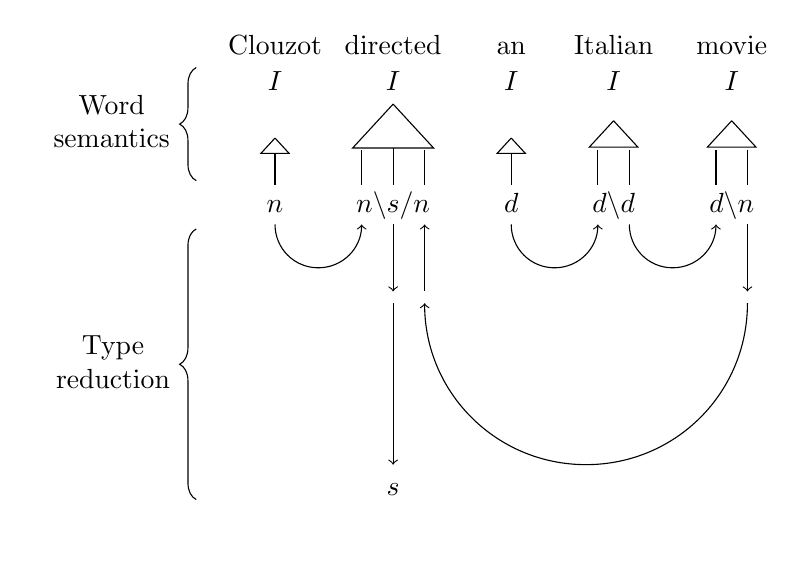
\begin{tikzpicture}[
every node/.style={%
text height=1.5ex,text depth=0.25ex,}]
% Diagram generated by http://github.com/wetneb/MorozParser
\makeatletter


\pgfdeclareshape{triangle}{
    \inheritsavedanchors[from=rectangle]
    \inheritanchorborder[from=rectangle]
    \inheritanchor[from=rectangle]{center}
    \inheritanchor[from=rectangle]{north}
    \inheritanchor[from=rectangle]{south}
    \inheritanchor[from=rectangle]{east}
    \inheritanchor[from=rectangle]{southwest}
    \inheritanchor[from=rectangle]{southeast}

    \backgroundpath{
        \southwest \pgf@xb=\pgf@x \pgf@yb=\pgf@y
        \northeast \pgf@xa=\pgf@x \pgf@ya=\pgf@y
        \pgf@xc=0.5\pgf@xa \advance\pgf@xc by+0.5\pgf@xb

        \pgfpathmoveto{\pgfpoint{\pgf@xc}{\pgf@ya}}
        \pgfpathlineto{\pgfpoint{\pgf@xb}{\pgf@yb}}
        \pgfpathlineto{\pgfpoint{\pgf@xa}{\pgf@yb}}
        \pgfpathlineto{\pgfpoint{\pgf@xc}{\pgf@ya}}
    }
}

\tikzstyle{big-triangle}=[triangle,draw,inner sep=0pt,minimum width=0.5cm,minimum height=0.15cm]
\tikzstyle{medium-triangle}=[big-triangle,scale=0.7]
\tikzstyle{vbig-triangle}=[big-triangle,scale=2]
\tikzstyle{mbig-triangle}=[big-triangle,scale=1.2]
\tikzstyle{small-triangle}=[big-triangle,scale=0.25]
\node at (0.0,0) (t2) {$n$};
\node at (0.0,2.0) (w0) {Clouzot};
\node at (1.5,0) (t8) {$n \backslash s / n$};
\node at (1.5,2.0) (w1) {directed};
\node at (3.0,0) (t17) {$d$};
\node at (3.0,2.0) (w2) {an};
\node at (4.3,0) (t28) {$d \backslash d$};
\node at (4.3,2.0) (w3) {Italian};
\node at (5.8,0) (t37) {$d \backslash n$};
\node at (5.800000000000001,2.0) (w4) {movie};

\node at (-1,2) (t) {};
\node at (-1,0.05) (b) {};
\draw[decorate,decoration={brace,amplitude=6pt}] (b) -- node[left] {\begin{tabular}{c} Word \\ semantics \end{tabular}} (t);

\node at (-1,-0.05) (t) {};
\node at (-1,-4) (b) {};
\draw[decorate,decoration={brace,amplitude=6pt}] (b) -- node[left] {\begin{tabular}{c} Type \\ reduction \end{tabular}} (t);

% Curves below :
\draw[->] (0.0,-0.25) .. controls (0.0,-0.55525) and (0.24474999999999997,-0.8) .. (0.55,-0.8) .. controls (0.8552500000000001,-0.8) and (1.1,-0.55525) .. (1.1,-0.25);

\draw[->] (3.0,-0.25) .. controls (3.0,-0.5552499999999999) and (3.24475,-0.7999999999999998) .. (3.55,-0.7999999999999998) .. controls (3.85525,-0.7999999999999998) and (4.1,-0.5552499999999999) .. (4.1,-0.25);

\draw[<-] (1.9,-0.25) -- (1.9,-1.1);
\draw[->] (6.0,-0.25) -- (6.0,-1.1);
\draw[->] (1.5,-0.25) -- (1.5,-1.1);

\draw[->] (4.5,-0.25) .. controls (4.5,-0.5552500000000002) and (4.744750000000001,-0.8000000000000003) .. (5.050000000000001,-0.8000000000000003) .. controls (5.355250000000001,-0.8000000000000003) and (5.6000000000000005,-0.5552500000000002) .. (5.6000000000000005,-0.25);

\draw[<-] (1.9,-1.25) .. controls (1.9,-2.3877500000000005) and (2.8122499999999997,-3.3000000000000007) .. (3.95,-3.3000000000000007) .. controls (5.087750000000001,-3.3000000000000007) and (6.000000000000001,-2.3877500000000005) .. (6.000000000000001,-1.25);

\draw[->] (1.5,-1.25) -- (1.5,-3.3000000000000007);
\node at (1.5,-3.6) {$s$};

% Curves above:

\node[medium-triangle] at (0.0,0.75) (fresh) {};
\node[above of=fresh] at (0.0,0.55) {$I$};
\draw (0.0,0.25) -- (fresh);

\draw (1.1,0.25) -- (1.1,0.7);
\node[vbig-triangle] at (1.5,1) (fresh) {};
\node[above of=fresh] at (1.5,0.55) {$I$};
\draw (1.5,0.25) -- (fresh);
\draw (1.9,0.25) -- (1.9,0.7);

\node[medium-triangle] at (3.0,0.75) (fresh) {};
\node[above of=fresh] at (3.0,0.55) {$I$};
\draw (3.0,0.25) -- (fresh);

\node[mbig-triangle] at (4.3,0.9) (fresh) {};
\node[above of=fresh] at (4.3,0.55) {$I$};
\draw (4.1,0.7) -- (4.1,0.25);
\draw (4.5,0.7) -- (4.5,0.25);

\node[mbig-triangle] at (5.8,0.9) (fresh) {};
\node[above of=fresh] at (5.8,0.55) {$I$};
\draw (5.6,0.7) -- (5.6,0.25);
\draw (6.0,0.7) -- (6.0,0.25);

\end{tikzpicture}

\end{figure}
